\newpage

\section{Time, Clocks, and Logical Ordering}
\subsection{Accuracy of Time: Atomic Clocks \& NTP}
\noindent
Time allows us to order and identify events. 
Say we ran \snippet{time.Now()} on two different machines:

\begin{figure}[h]
    \centering
    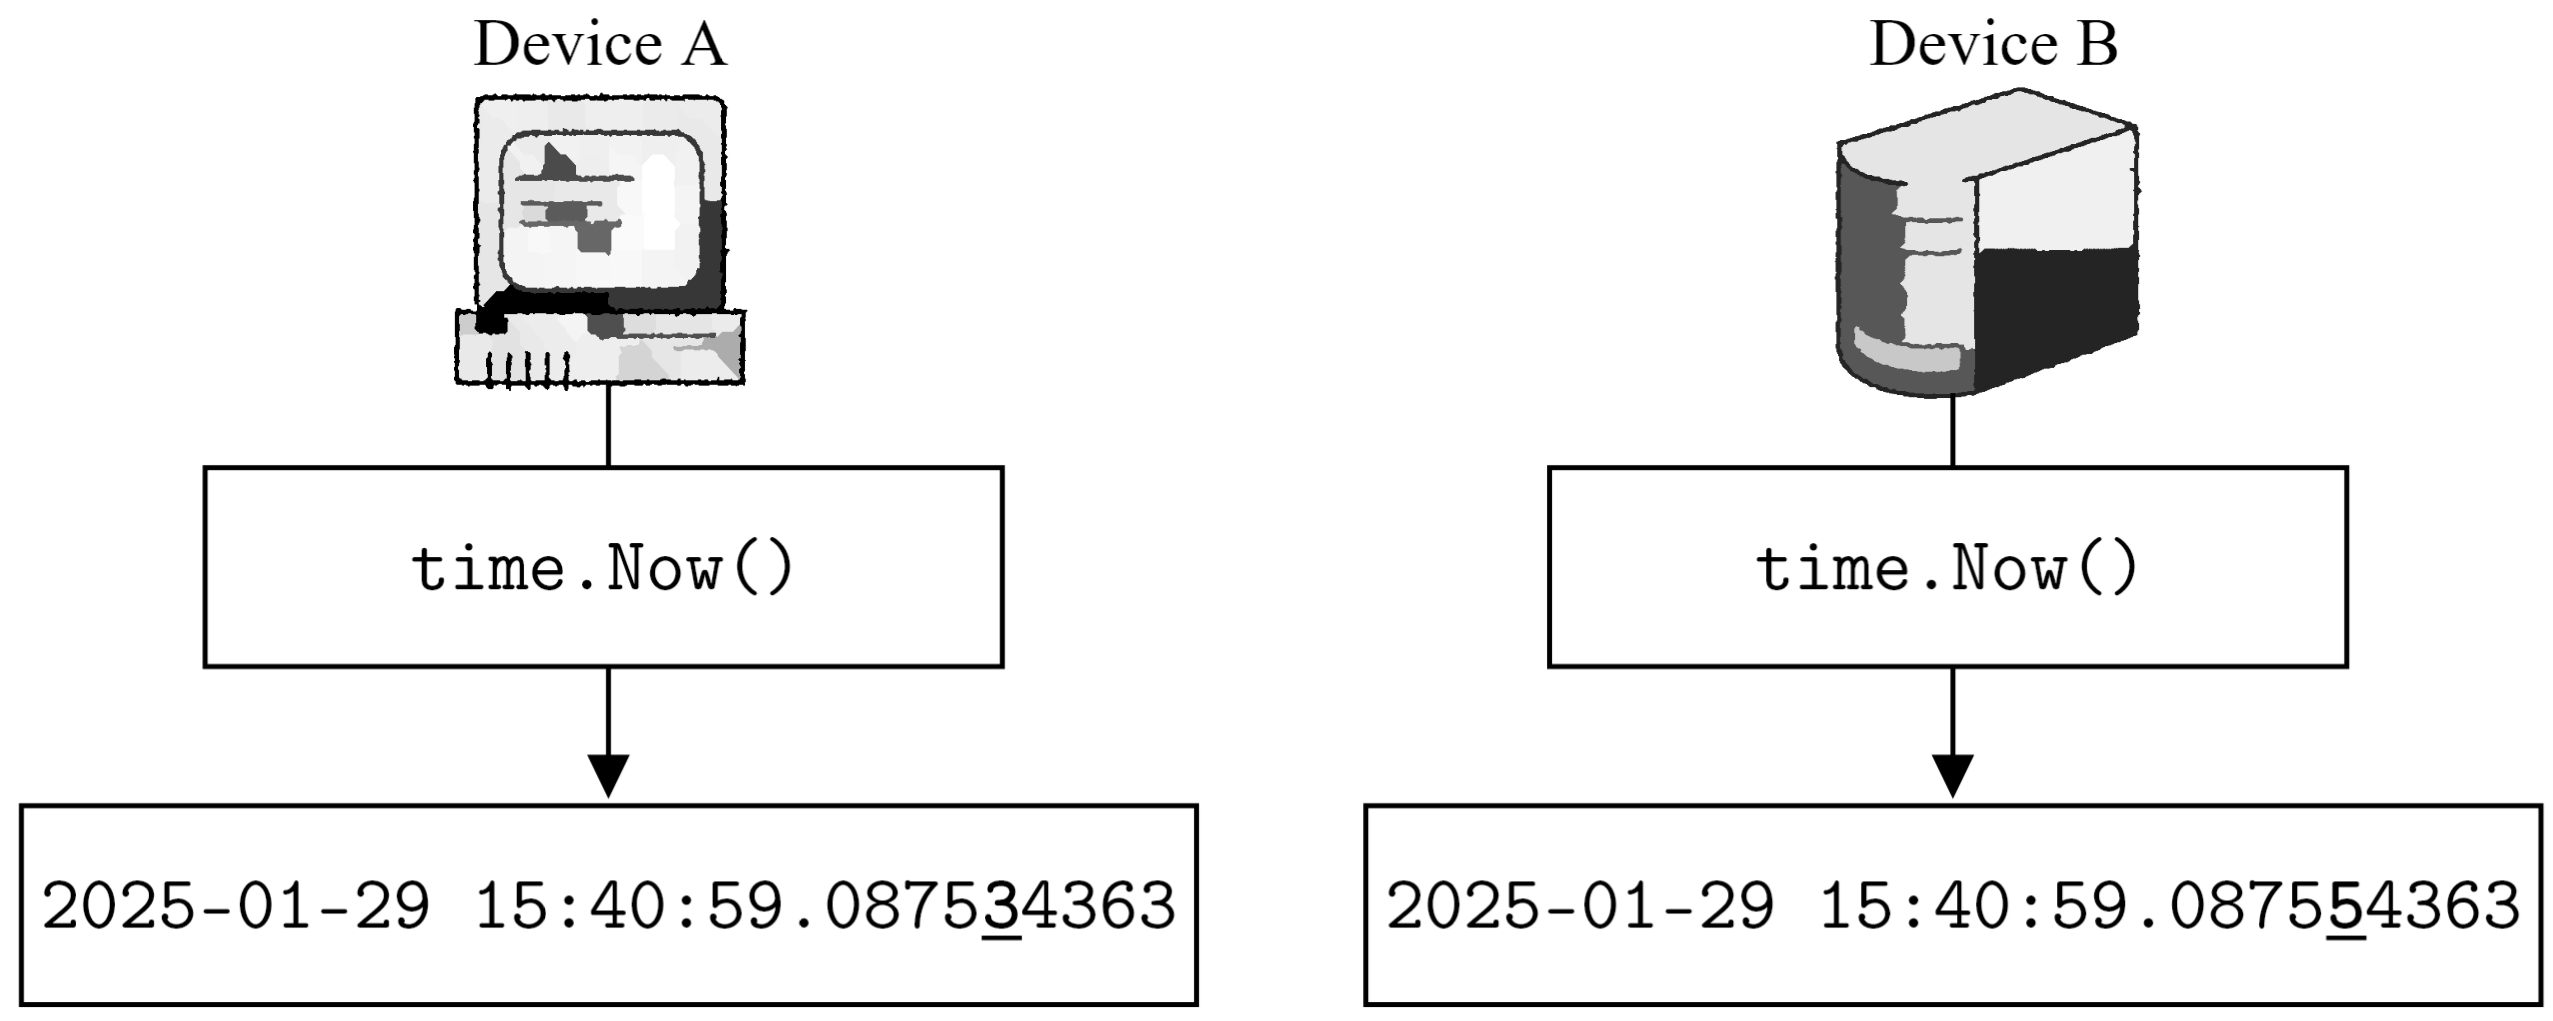
\includegraphics[width=.9\textwidth]{./Sections/time/now.png}
    \caption{Using \snippet{time.Now()} on two different machines}
\end{figure}

\noindent
Despite Device $A$ appearing to be ahead of Device $B$, we cannot be certain via 
the following reasons:

\begin{theo}[Clock Synchronization Impossibility]

    There are two key reasons why perfect clock synchronization is impossible:

    \begin{itemize}
        \item \textbf{Clock Skew:} There's a difference between every system clock (ideally 0), as they maintain their own local clock via a hardware oscillator incrementing a counter register.
        \item \textbf{Clock Drift:} Even if systems initialize with a reference time, their clocks will inevitably diverge due to variations in manufacturing, age, or environmental factors such as temperature.
        We measure the deviation by, $\dfrac{dC}{dt}=1+\rho$, where $C$ is the clock time and $t$ is the real time, and $\rho$ (rho) is the drift rate (ideally 0).
    \end{itemize}
\end{theo}

\noindent
We may formalize what we may consider synchronized clocks as follows:
\begin{Def}[Clock Synchronization Threshold]
    
    Let there be two clocks $C_i$ and $C_j$. They are (delta) $\delta$-synchronized if for all $t$ time units:
    \[ |C_i(t) - C_j(t)| \leq \delta \]

    \noindent
    \textbf{E.g.,} $C_i$ and $C_j$ are $\delta$-synchronized within 10ms if $|C_i(t) - C_j(t)| \leq 10ms$
\end{Def}

\newpage 

\noindent
In practice we to achieve semi-synchronized clocks, we developed the following protocol:

\begin{Def}[Network Time Protocol (NTP)]
    
    The NTP is a protocol synchronizes network clocks via a ground-truth time distribution system.
    The ground-truth time is are GPS satellite \textbf{atomic clocks}, which exhibit negligible drift over millions of years.

    NTP employs a \textbf{round-trip time (RTT)} calculation to estimate the clock offset request latency. 
    It also organizes synchronization strength into a \textbf{stratum hierarchy}, where lower-numbered stratums indicate more accurate time sources:

    \begin{itemize}
        \item \textbf{Stratum 0:} Ground truth \textbf{atomic clocks}/\textbf{GPS receivers}.
        \item \textbf{Stratum 1:} NTP servers that directly synchronize with Stratum 0 reference clocks.
        \item \textbf{Stratum 2:} NTP servers synchronized to Stratum 1 servers.
        \item \textbf{Stratum 3 and beyond:} Weaker NTP servers synchronized to higher-stratum servers.
        \item \textbf{Stratum 16:} A system considered \textit{unsynchronized} (e.g., a freshly booted system).
    \end{itemize}
\end{Def}

\vspace{-1em}
\begin{figure}[h]
    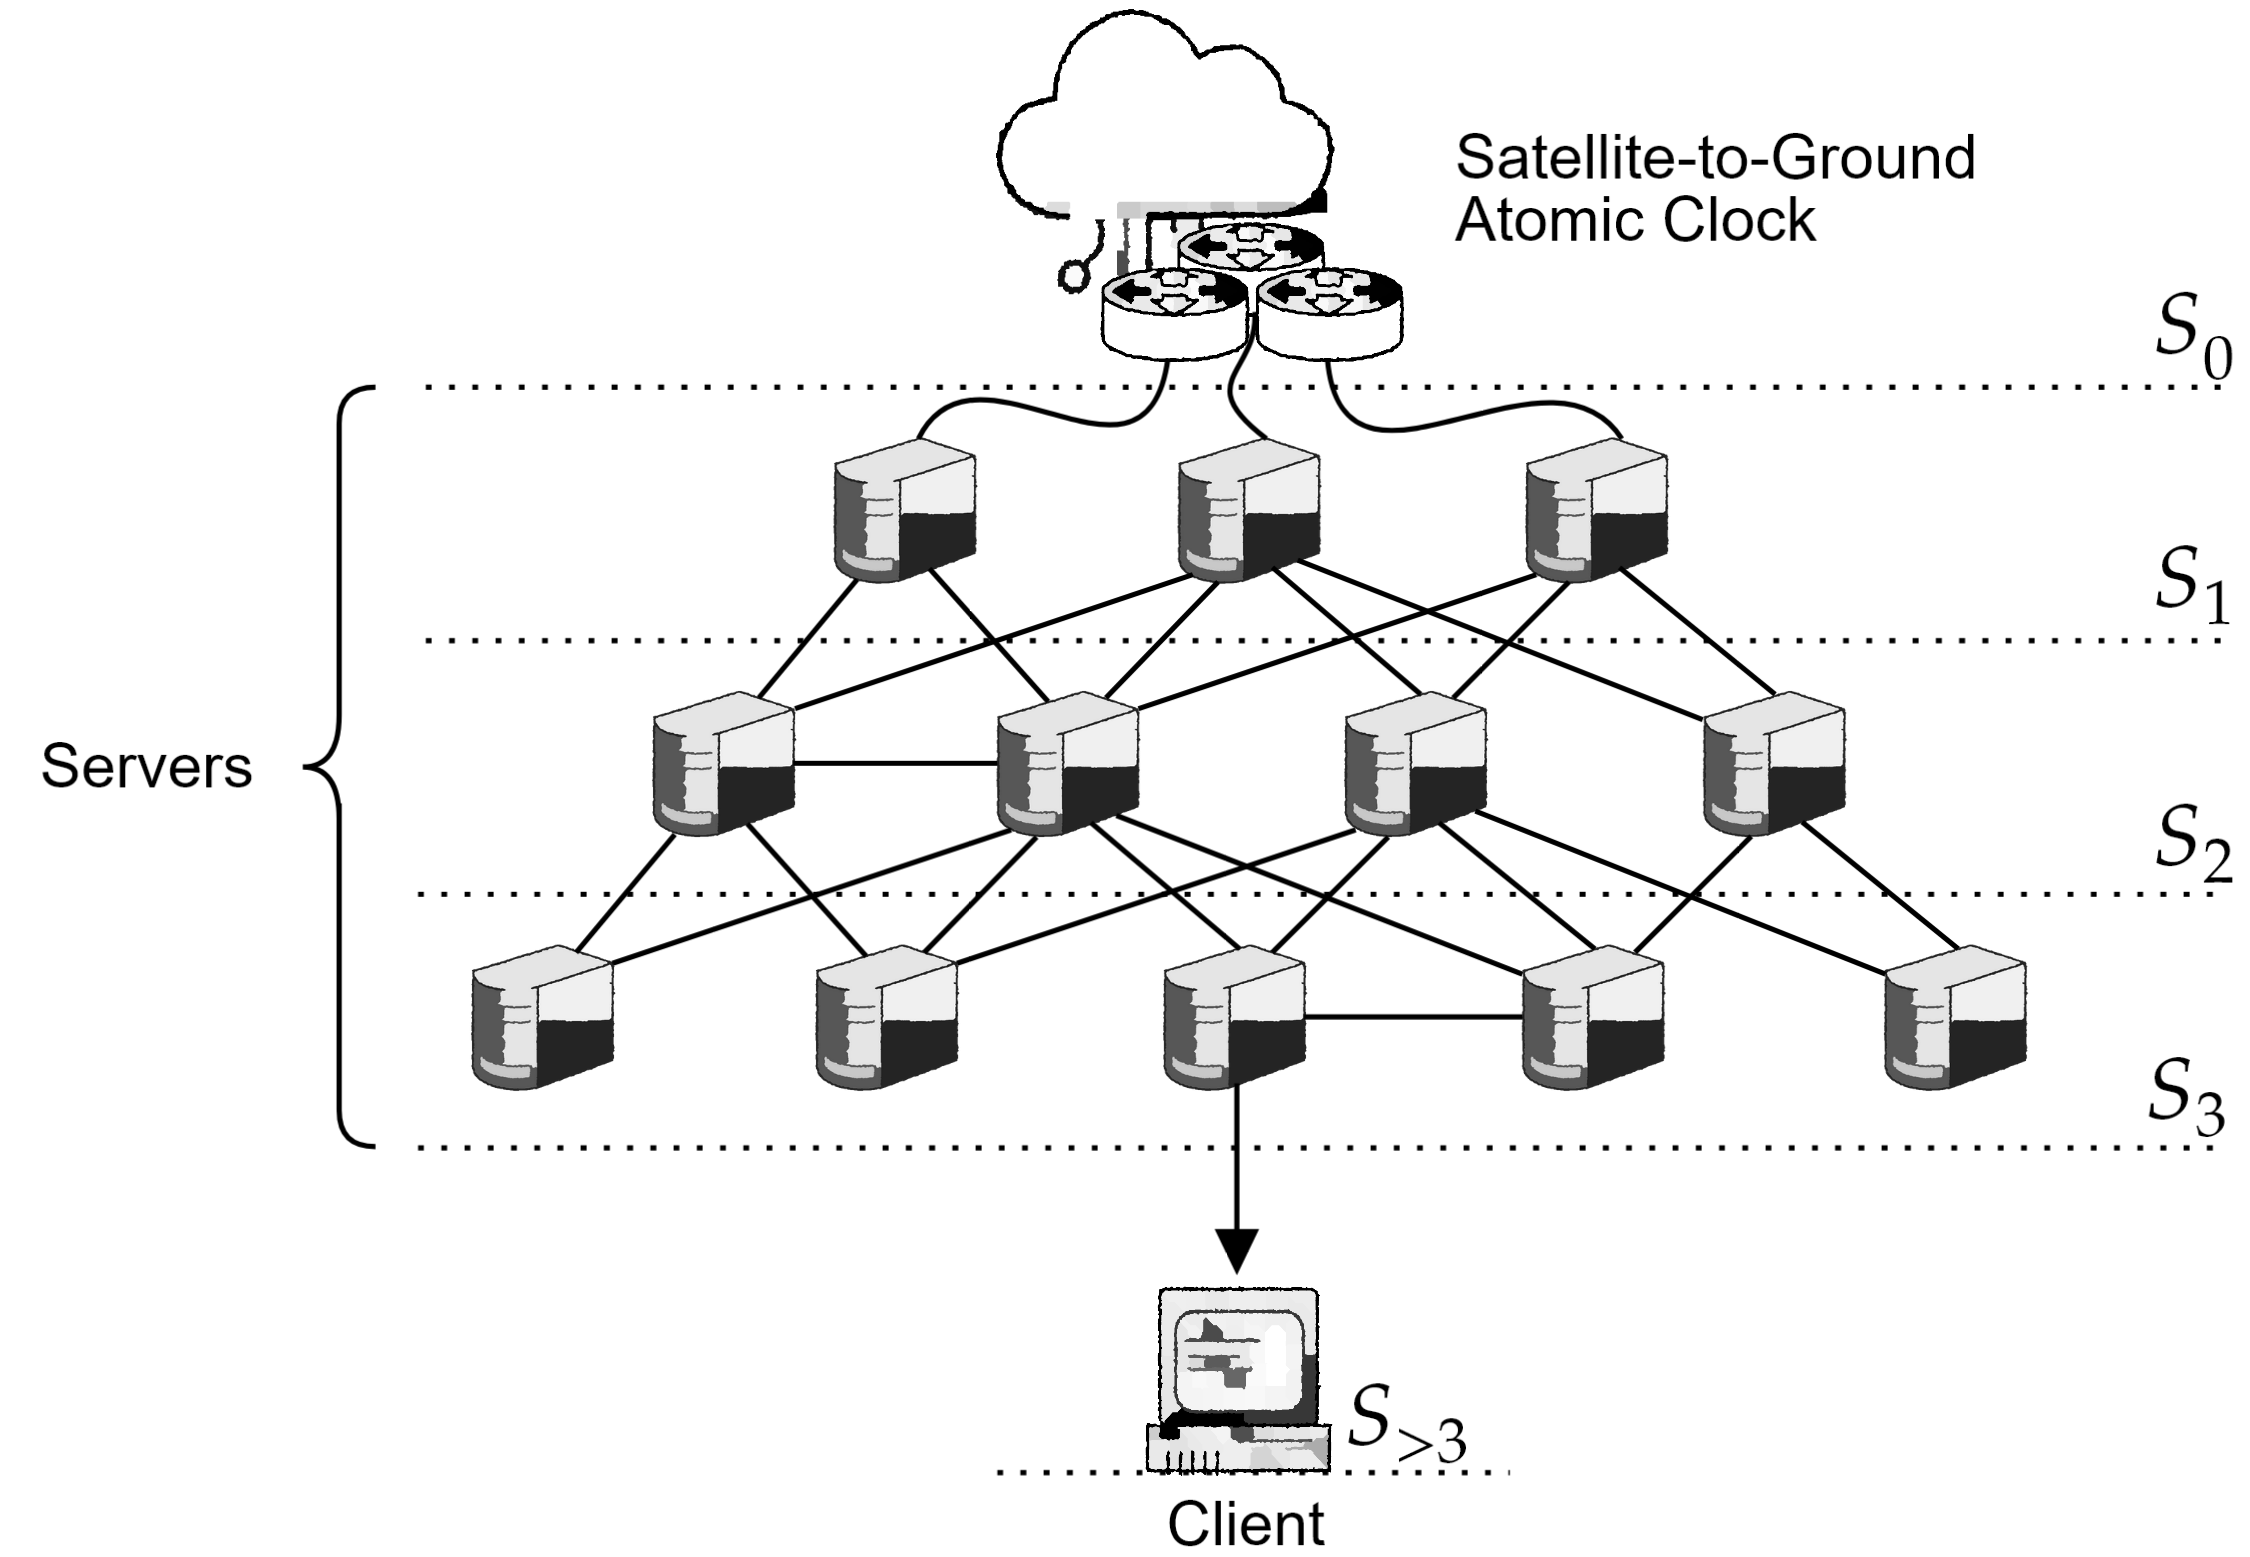
\includegraphics[width=.9\textwidth]{./Sections/time/sat.png}
    \caption{NTP Stratum Hierarchy From GPS Satellite Atomic Clock to Client.}
\end{figure}

\newpage 
\subsection{Logical Clocks: Lamport \& Vector Clocks}

\noindent
To get away from the limitations of physical clocks, we may use logical clocks to order events.

\begin{Def}[Logical Clocks]

    Let $a$ and $b$ be two events part of a totally ordered set of events. Let function $t(x)$ denote the time of event $x$. Then,
    \[ a \rightarrow b \implies t(a) < t(b) \]

    \noindent
    Where $a \rightarrow b$ denotes that event $a$ happens before $b$, which implies $t(a) < t(b)$.
\end{Def}

\noindent
We may become more formal about cause and effect relationships with the following definition:
\begin{Def}[Causal Order]

    For $r$ \textbf{execution trace} (sequence of events), the causal order relationship $\rightarrow_r$ is defined as:

    \begin{itemize}
        \item If $a$ \textbf{happens before} $b$ in the same process, then $a \rightarrow_r b$.
        \item If $a$ is a \textbf{sender} and $b$ the \textbf{receiver}, then $a \rightarrow_r b$.
        \item \textbf{Transitive Property}: if $a \rightarrow_r b$ and $b \rightarrow_r c$, then $a \rightarrow_r c$.
        \item Events $a$ and $b$ are \textbf{concurrent} (denoted as $a \parallel b$) if:
            \begin{itemize}
                \item[$\blacktriangleright$] $a \not\rightarrow_r b$ and $b \not\rightarrow_r a$, meaning neither event happened before the other.
            \end{itemize}
    \end{itemize}
\end{Def}
\begin{Example}[Causal Order Example]

    \label{ex:causal}
    Determine the causal order relationship between events in processes $P$ and $P'$:

    \begin{itemize}
        \item (a): $a\ ?\ b;\quad $ (b): $a\ ?\ k;\quad$ (c): $ c\ ?\ b;\quad$ (d): $ c\ ?\ e$
    \end{itemize}

    

    \hspace{4em}
    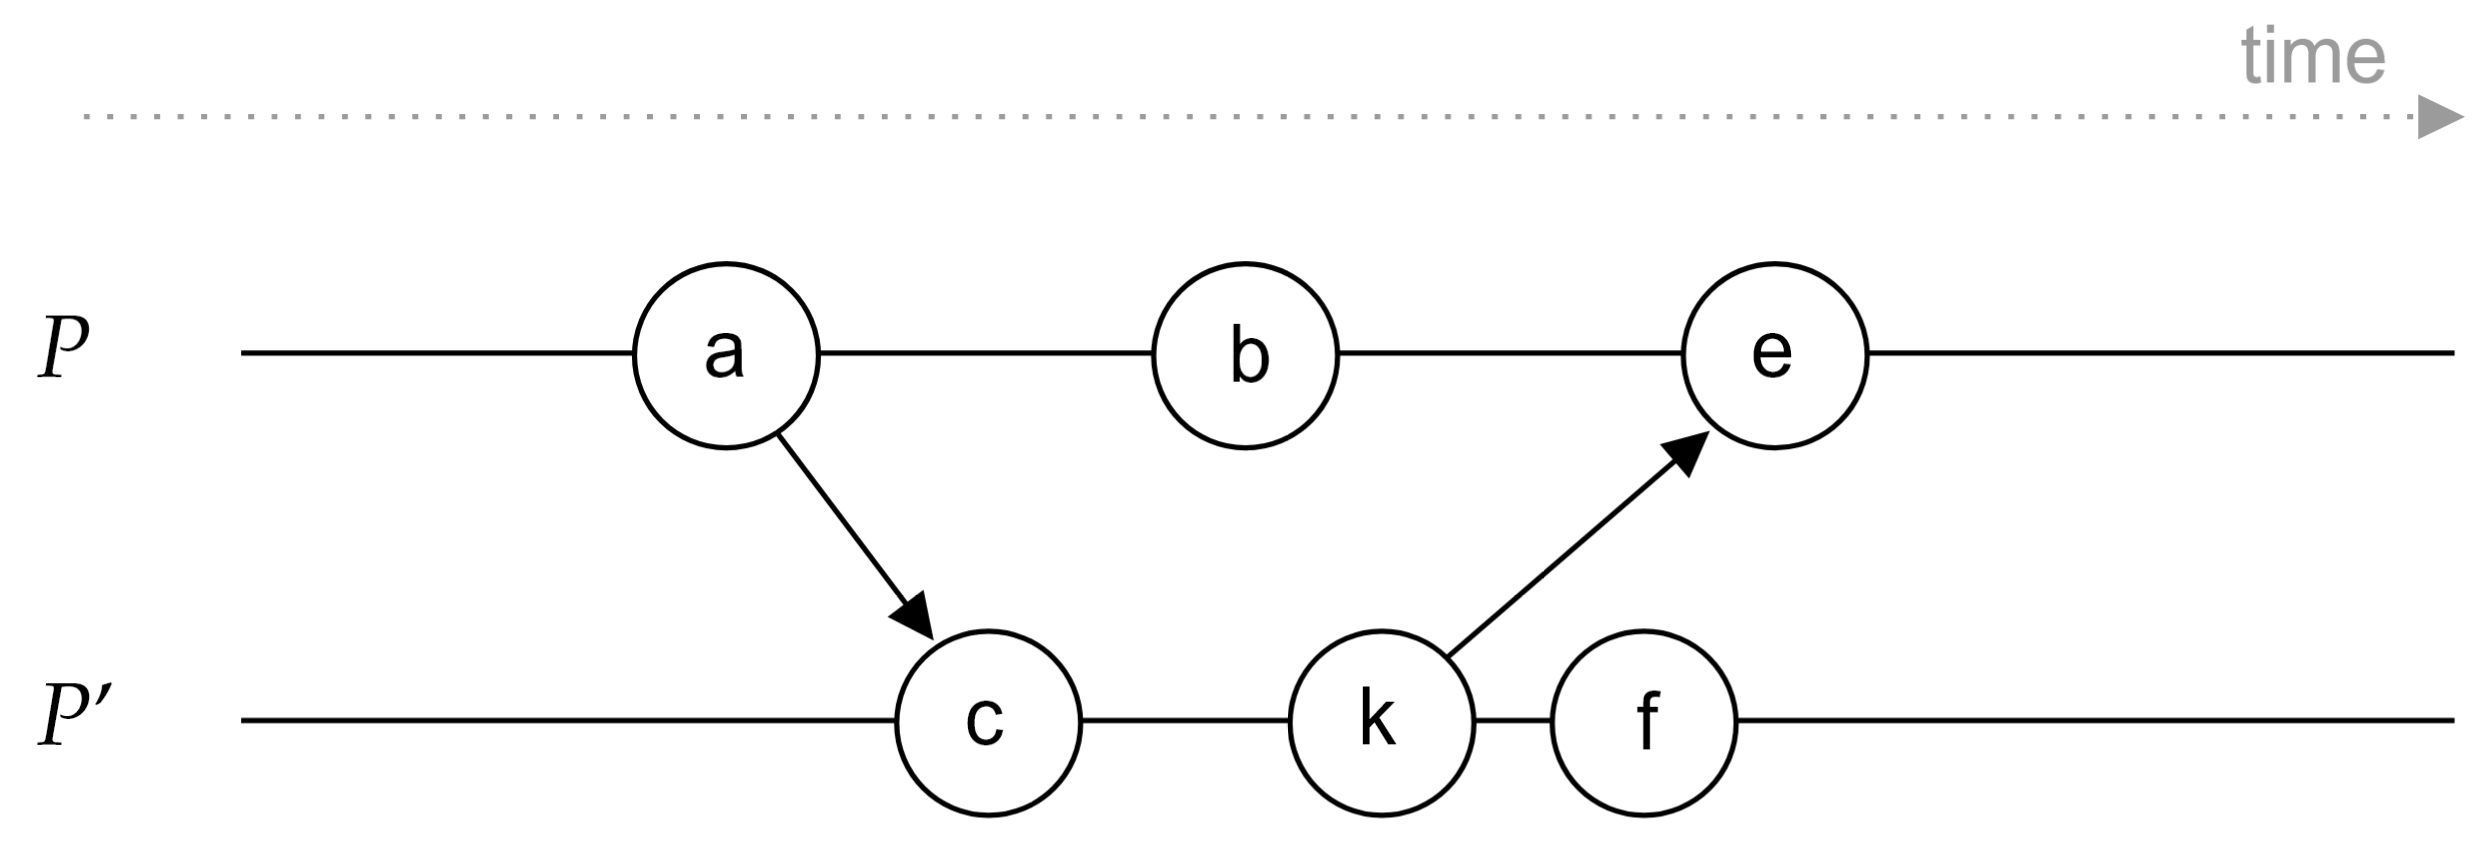
\includegraphics[width=.7\textwidth]{./Sections/time/causal.png}
        
    \vspace{1em}
    \noindent
    Answer on the next page.
\end{Example}
\newpage 

\noindent
\textbf{Example (\ref{ex:causal}) Answer:} (a): $a \rightarrow_r b$;\quad (b): $a \rightarrow_r k$;\quad (c): $c \parallel b$;\quad (d): $c \rightarrow_r e$.\\
\noindent
\rule{\textwidth}{0.4pt}\\

\noindent
Now we discuss a method that utilizes causal order, though assigns logical timestamps to events:
\begin{Def}[Lamport Clocks]

    Named after Leslie Lamport, Lamport Clocks assign a logical timestamp to each event:\\
    
    \noindent
    Let $t_p$ store the logical time of process $p$. Then,
    \begin{itemize}
        \item \textbf{Initialization:} $t_p$ is initialized to 0.
        \item \textbf{Timestamp Syntax:} Timestamps are tuples $(t_p, p)$, assigned to each $e$ event.
        \item \textbf{Incrementing:} For each $e$ in process $p$, increment $t_p$ by 1 and assign the $(t_p, p)$ to $e$.
        \item \textbf{Sending:} If $p$ sends a message $m$ to process $q$, the timestamp included is $((t_p+1), p)$.
        \item \textbf{Receiving:} Upon receiving message $m$, process $q$ sets $t_q = \max((t_p+1),t_q)$.
    \end{itemize}
\end{Def}

\begin{Example}[Lamport Clocks Example (\ref{ex:causal}) Extended]

    Consider the previous Example (\ref{ex:causal}) with Lamport Clocks:

    \hspace{4em}
    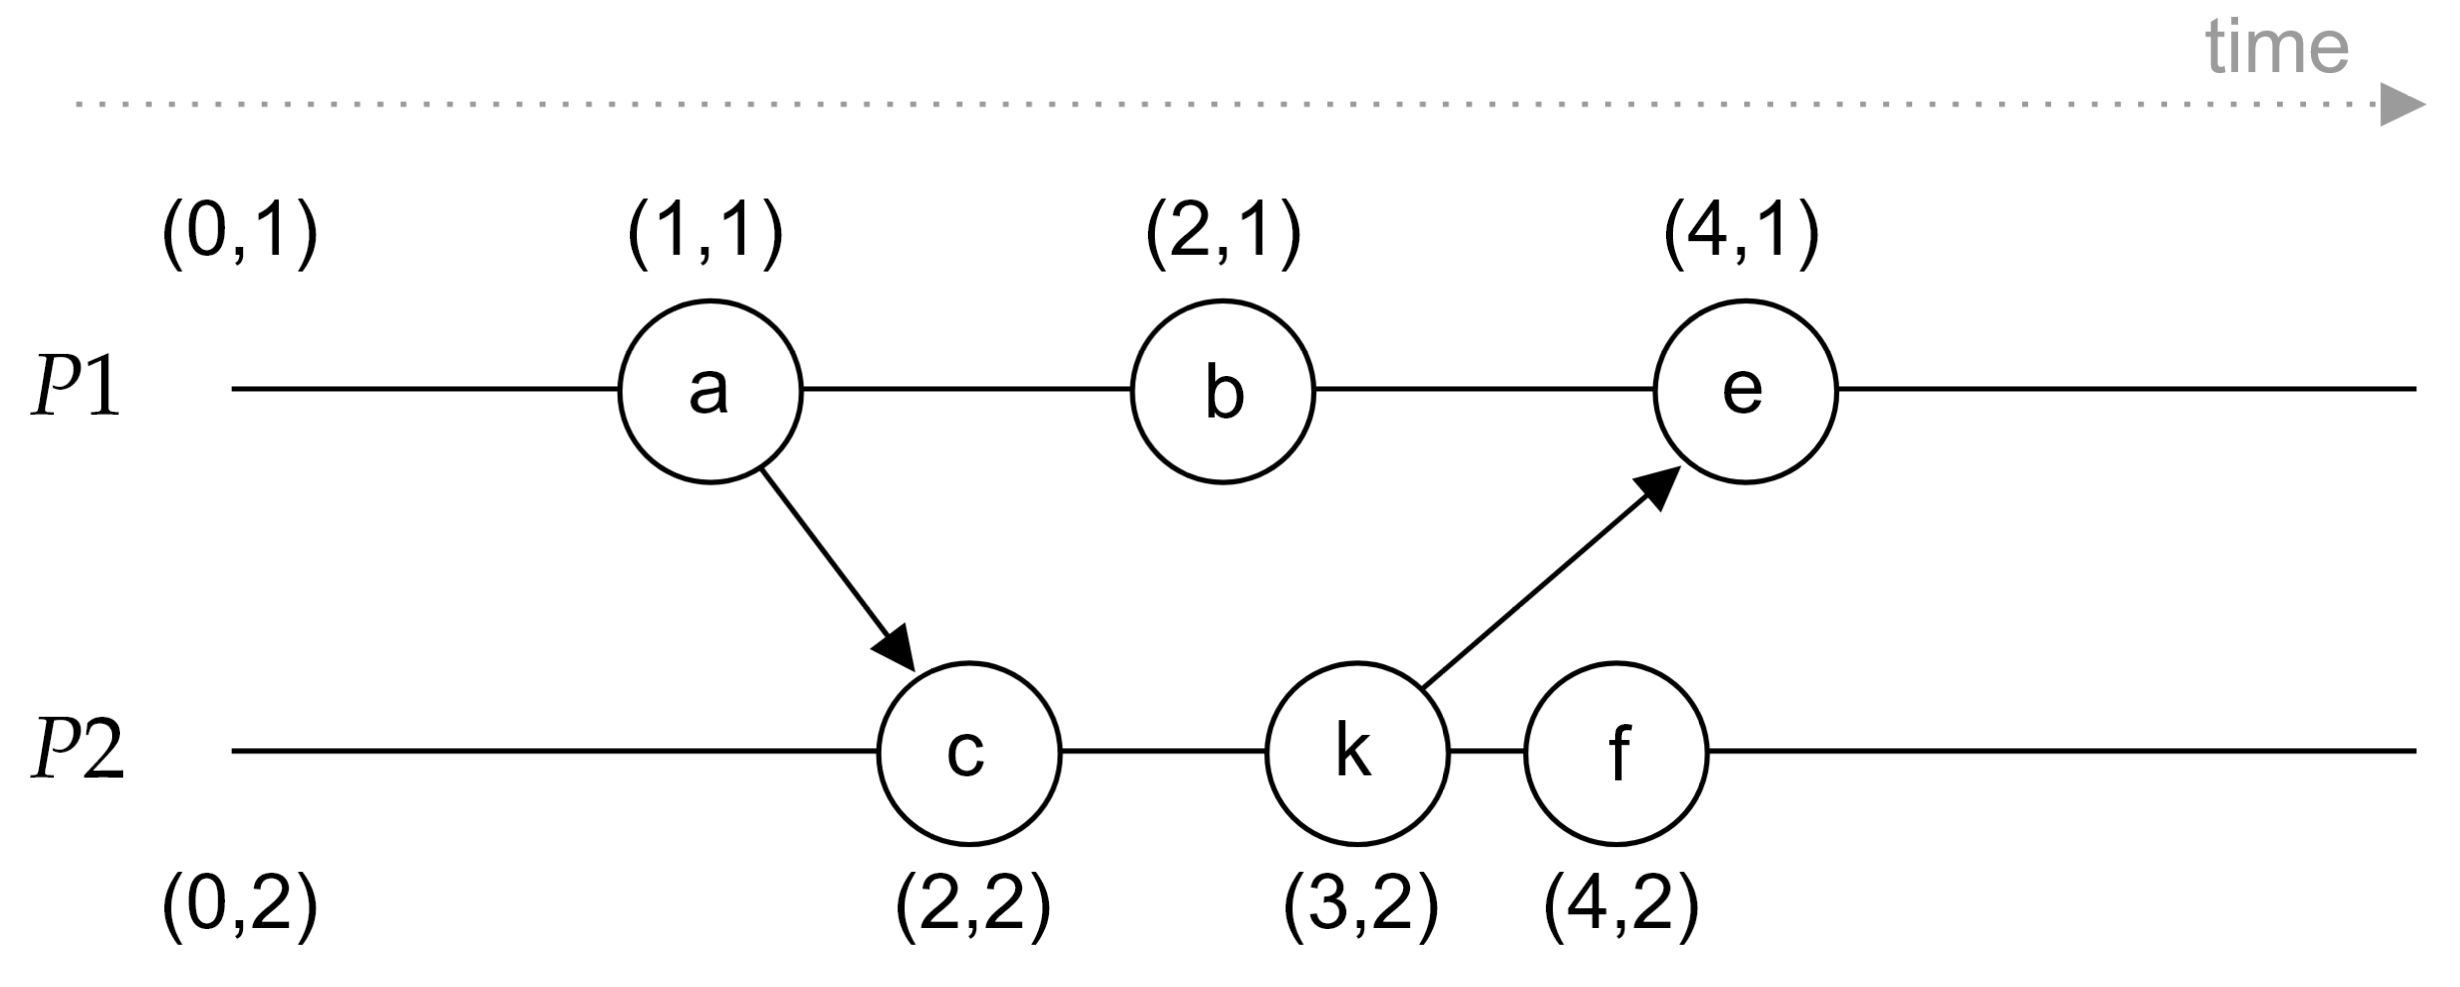
\includegraphics[width=.7\textwidth]{./Sections/time/lamport.png}

\end{Example}

\noindent
In practice the only thing we have access to are these logical timestamps, which we must evaluate:
\begin{theo}[Comparing Lamport Timestamps]

    Given two events $a$ and $b$ with timestamps $t(a)$ and $t(b)$, with $r$ trace, we only guarantee:
    \begin{itemize}
        \item If $a \rightarrow_r b$, then $t(a) < t(b)$.
        \item If $t(a) \geq t(b)$, then $a \not\rightarrow_r b$.
    \end{itemize}
\end{theo}

\newpage 

\noindent
We may now derive the following about concurrency:
\begin{theo}[Non-causality]

    Two events $a$ and $b$ are concurrent ($a \parallel b$) under $r$ trace if \textbf{both} conditions 
    hold:
    \begin{itemize}
        \item $a \not\rightarrow_r b$ ($a$ does not happen before $b$).
        \item $b \not\rightarrow_r a$ ($b$ does not happen before $a$).
    \end{itemize}
\end{theo}

\noindent
Lamport Clocks are useful for causal ordering, but they do not capture the full context of events:
\begin{Def}[Vector Clocks]

   Let there be $p_1, p_2, \ldots, p_n$ processes each with a vector (array) $v$ of size $n$. Each index $v[i]$ stores the logical time of process $p_i$.
   Then, the following rules apply:
   \begin{itemize}
    \item \textbf{Initialization:} Each $v[i]$ of $p_i$ is initialized to 0 (e.g., $[0,0,\dots,0]$).
    \item \textbf{Incrementing:} For each event $e$ in process $p_i$, increment $v[i]$ by 1.
    \item \textbf{Sending:} When $p_i$ sends a message $m$ to $p_j$, include $v$ in $m$ (\textbf{no increment}).
    \item \textbf{Receiving:} Upon receiving message $m$, process $p_j$ sets $v[j] = \max(v[j], m[j])$.
   \end{itemize}
\end{Def}
